En este capítulo se describen distintos enfoques software a la hora de explotar el paralelismo 
existente en las arquitecturas paralelas más extendidas actualmente, incluyendo sistemas multinúcleo y 
arquitecturas heterogéneas, haciendo especial hincapié en los mecanismos existentes a la hora de
explotar sistemas asimétricos. Se describen las dos soluciones con mayor aceptación a día de hoy. 
La Sección~\ref{sec:tareas} introduce los mecanismos e implementaciones más extendidas para la
extracción y explotación de paralelismo a nivel de tareas. 
La Sección~\ref{sec:bibliotecas} incide en el desarrollo de bibliotecas paralelas, extrayendo
paralelismo a nivel de datos.
En ambos casos, se tomará como hilo conductor un ámbito concreto: el desarrollo de códigos matemáticos
dentro del ámbito del álgebra lineal, ya que serán estos códigos los utilizados en la descripción
del trabajo realizado en próximos capítulos.
Finalmente, la Sección~\ref{sec:comparativa} realiza una breve comparativa entre ambos enfoques,
destacando las ventajas e inconvenientes de cada uno de ellos desde el punto de vista del rendimiento
y de la facilidad de programación.


\section{Modelos de programación basados en paralelismo a nivel de tareas}
\label{sec:tareas}

El DAG asociado con un algoritmo o rutina es una representación gráfica del paralelismo de tareas asociado a ella,
e, idealmente, un planificador de tareas en tiempo de ejecución podría explotar esta información para determinar
distintas planificaciones (esto es, ordenación de tareas y asignación de las mismas a recursos computacionales
disponibles) que satisfacen las dependencias fijadas en el DAG.

\subsection{Introducción al paralelismo a nivel de tareas. Estado del arte}

Los modelos de programación basados en la extracción de paralelismo a nivel de tareas han demostrado
su utilidad, particularmente en el campo del álgebra lineal~\cite{Abalenkovs}. En general, el objetivo
principal radica en proporcionar al programador algún mecanismo para permitir expresar el paralelismo
potencial a nivel de tareas existente en la aplicación, normalmente en forma de grafo de tareas, más un
planificador de tareas (o runtime) que realice una planificación dinámica de las mismas, respetando
las dependencias de datos entre ellas y a la vez permitiendo un correcto aprovechamiento
de las unidades de procesamiento disponibles.

Entre las propuestas e implementaciones más extendidas para este tipo de modelo de programación cabe
destacar, entre otros, Cilk Plus, StarPU, Superglue, QUARK, Kaapi y OmpSs. 

Cilk Plus~\cite{cilkweb,Blumofe:Cilk,Frigo:Cilk,Leiserson:Cilk} es un lenguaje diseñado exclusivamente
para programación paralela basado en C, con extensiones que permiten expresar tanto el paralelismo a nivel
de tareas como a nivel de datos. Cilk incorpora un componente software para la planificación de tareas
en tiempo de ejecución aprovechando el paralelismo expuesto por el programador. Fue desarrollado en los
años 90 en el MIT, distribuido de forma comercial más tarde por Intel, y liberado e integrado en proyectos
de software libre (por ejemplo, GCC) más tarde. En su versión actual, Cilk no incorpora ningún soporte 
específico para arquitecturas heterogénelas ni asimétricas.

StarPU~\cite{starpuweb,Augonnet:2011:SUP:1951453.1951454,agullo:hal-01223573,agullo:hal-01120507} implementa un planificador de tareas en tiempo de ejecución y soporte de cara al programador
a la hora de anotar tareas mediante pequeños fragmentos de código ({\em codelets}). Aunque el runtime se ha
aplicado frecuentemente a la resolución de algoritmos numéricos, es de carácter generalista, y gestiona
las transferencias de datos entre espacios de memoria (en arquiteturas heterogéneas) mediante
una biblioteca que fuerza la coherencia de memoria e incluye prebúsqueda automática de datos.

Superglue~\cite{superglueweb,tillenius:superglue,tillenius:superglue2} es también un modelo basado en tareas, en el que las
dependencias de datos se represetan usando versiones en lugar de grafos de dependencias. El runtime 
realiza la planificación de las tareas considerando que todos los procesadores
son idénticos, pero tiene en cuenta el uso de recursos de cada tarea para evitar problemas
de contención.

Quark ({\em QUeing And Runtime for Kernels})~\cite{quarkweb,icl:609,Haidar} es un runtime que permite la 
ejecución dinámica de tareas con depedencias de datos en sistemas multinúcleo
con memoria compartida; forma parte de la biblioteca de álgebra lineal PLASMA~\cite{Abalenkovs}.

Kaapi ({\em Kernel for Adaptive, Asynchronous Parallel and Interactive Programming})~\cite{kaapiweb,Gautier:2013:XRS:2510661.2511383,Gautier:2007:KTS:1278177.1278182}
es una biblioteca C++ para programación basada en tareas similar a Cilk, desarrollada en el INRIA.
Existen versiones de su planificador tanto para sistemas multihebra como multi-GPU (XKaapi), cuyo
modelo de programación permite crear tareas de forma similar a Cilk, StarSs u OmpSs. El paralelismo
es explícito y las dependencias entre tareas y transferencias entre espacios de memoria son 
gestionadas automáticamente por el planificador.

%\begin{itemize}
%
%\item Hacer un repaso por las distintas alternativas en planificadores a nivel de tareas existentes.
%
%\item Hacer hincapié en el soporte para arquitecturas heterogéneas (muchos lo soportan).
%
%\item Destacar el poco soporte para arquitecturas asimétricas, lo que da valor a nuestra propuesta.
%
%\end{itemize}

\subsection{OmpSs. Modelo de programación y planificación de tareas}

OmpSs es uno de los modelos de programación paralela a nivel de tareas más
extendidos a día de hoy. A grandes rasgos, el diseño del modelo de
programación se basa en la inclusión de directivas (o {\tt pragma}s)
similares a las utilizadas en otros modelos de programación paralela, como
OpenMP. Sin embargo, dichas directivas se limitan en su mayoría, a la
anotación de ciertos bloques de código (típicamente funciones) para
informar de su carácter de {\em tareas}, es decir, unidades básicas de
planificación a los recursos computacionales disponibles. Dicha
planificación se difiere hasta el momento de la ejecución del código, en el
que un {\em planificador de tareas} o {\em runtime} (en el caso de OmpSs,
llamado Nanox) se encarga de mapear, de forma eficiente, su ejecución al
mejor recurso computacional disponible en un momento dado.

\subsubsection{El modelo de programación OmpSs}

Con el fin de ayudar al programador en la construcción de un DAG completo y
correcto partiendo de un código secuencial, OmpSs proporciona mecanismos
sencillos y no invasivos. En dicho modelo, el programador utiliza
directivas similares a OpenMP ({\tt pragma}s) para anotar rutinas
existentes en el código como tareas, indicando a la vez la direccionalidad
de sus operandos (entrada, salida o entrada/salida) a través de cláusulas
adicionales. A grandes rasgos, el planificador de OmpSs descompone el
código (transformado previamente a través del compilador fuente-a-fuente
Mercurium~\cite{Mercurium}) en un conjunto de tareas, identificando las
dependencias entre ellas, y lanzando a ejecución únicamente {\em tareas
  listas} (es decir, aquellas cuyas dependencias han sido satisfechas) para
su ejecución en los distintos núcleos computacionales del
sistema. Adicionalmente a las directivas proporcionadas para la creación de
tareas, OmpSs proporciona un conjunto de directivas orientadas a la
sincronización de las distintas tareas.

\subsubsection{Planificación de tareas en OmpSs. El \emph{runtime} Nanox}

Una vez que un código anotado ha sido compilado con el compilador de OmpSs
Mercurium, este puede ser ejecutado a través del \emph{runtime} de OmpSs
denominado Nanox, consistente en una serie de librerías encargadas de
controlar la ejecución del programa e intentar finalizar la ejecución de la
manera más eficiente posible. Para ello, Nanox está compuesto por un núcleo
principal encargado de la gestión de los distintos hilos y estructuras
internas, y un conjunto de módulos encargados de distintas tareas como
puede ser el módulo encargado de la planificación de las tareas sobre los
hilos, el módulo encargado de comprobar las dependencias entre tareas, o el
módulo encargado de obtener distintas trazas durante la ejecución.

Una vez que un programa anotado es lanzado sobre Nanox, éste realiza una
serie de pasos para inicializar el \emph{runtime} antes de comenzar la
ejecución del programa original. Entre estos pasos, uno de ellos es la
creación de un número fijo de hilos denominados \wts, los cuales van a ser
los encargados de ejecutar las distintas tareas que estén listas para
ejecución (el número de hilos creados es escogido por el usuario en el
momento de iniciar la ejecución). El primero de estos \wts creados, a parte
de ejecutar tareas igual que el resto de \wts, también es el encargado de
ejecutar el código secuencial del programa, por lo que mientras que el
resto de hilos pueden estar ociosos en el caso de no existir ninguna tarea
lista para ejecución, este hilo siempre estará ejecutando ocupado. Notar
que al contrario que en el modelo de ejecución usado por OpenMP, Nanox no
crea un nuevo hilo por cada tarea a ejecutar, sino que crea un conjunto de
hilos al inicio de la aplicación, y son estos los encargados de ejecutar
todas las tareas del programa, finalizando su vida al acabar la ejecución
del mismo.

Cuando un \wt finaliza la ejecución de una tarea, este realiza dos acciones
sobre el \emph{runtime}:
\begin{enumerate}
\item El \wt informa al \emph{runtime} de la finalización de la tarea. Al
  finalizar la tarea, el módulo encargado de comprobar las dependencias
  comprueba qué nuevas tareas están listas para ser ejecutadas ya que se
  han satisfecho todas sus dependencias. Cuando se determina que una tarea
  está lista para ejecución, se informa al módulo encargado del
  planificador para que la almacene y trate de acuerdo a la política que
  implemente el módulo cargado.
\item El \wt solicita una nueva tarea para ejecutar al módulo
  planificador. El módulo planificador, en función de la política que se
  haya decidido usar, y del \wt que solicite la tarea, decidirá qué tarea
  debe ejecutar. En caso de no existir ninguna tarea lista para ejecutar, o
  el \wt no sea el idóneo para ejecutar ninguna de las tareas listas
  existentes, este pasa a estado inactivo hasta la creación de nuevas
  tareas, evitando así consumir recursos de manera innecesaria.
\end{enumerate}

La forma en la que se crean nuevas tareas corresponde al momento en el que
un \wt en ejecución se encuentra una anotación para la creación de una
nueva tarea. En este momento, \wt informa al \emph{runtime} para que cree
la tarea correspondiente y la inserte al DAG del problema, esperando a que
todas sus dependencias sean satisfechas y la nueva tarea esté lista para su
ejecución.



\subsection{Ejemplo: paralelización de la factorización de Cholesky}

A continuación describimos los mecanismos utilizados para extraer paralelismo a nivel de tareas
durante la ejecución de una operación específica de álgebra lineal densa, utilizando la Factorización
de Cholesky como hilo conductor. Esta operación en particular es representativa de muchas
otras factorizaciones utilizadas en la resolución de sistemas lineales, por lo que gran parte de las
conclusiones extraídas sobre ella pueden ser aplicadas a otro tipo de operaciones similares ampliamente
utilizadas en ciencia e ingeniería.
%
La Factorización de Cholesky descompone una matriz simétrica definida positiva
$A$ en el producto $A=U^TU$, donde el factor de Cholesky $U$ de dimensión $n \times n$ es una matriz triangular
superior~\cite{GVL3}. 

\lstinputlisting[float=th!,frame=lines,caption=Implementación en lenguaje C de la factorización de Cholesky orientada a bloques.,label=lst:chol]{Codes/cholesky.c}

El código de la Figura~\ref{lst:chol} muestra un código simplificado en lenguaje C para
la factorización de una matriz {\tt A} de dimensiones {\tt n}$\times${\tt n}, 
almacenada como un conjunto de {\tt s}$\times${\tt s} submatrices (bloques de datos) de dimensíón 
{\tt b}$\times${\tt b}.

Esta rutina orientada a bloques descompone la operación global en una colección de kernels u operaciones
fundamentales:
{\tt po\_cholesky} (Factorización de Cholesky), {\tt tr\_solve} (resolución de un sistema triangular),
{\tt ge\_multiply} (multiplicación de matrices), y 
{\tt sy\_update} (actualización simétrica de rango-{\tt b}), que operan sobre cada bloque
de datos de la matriz, y forman parte de las rutinas proporcionadas por los estándares LAPACK y BLAS. 

\begin{figure}%[tbh!]
\begin{center}
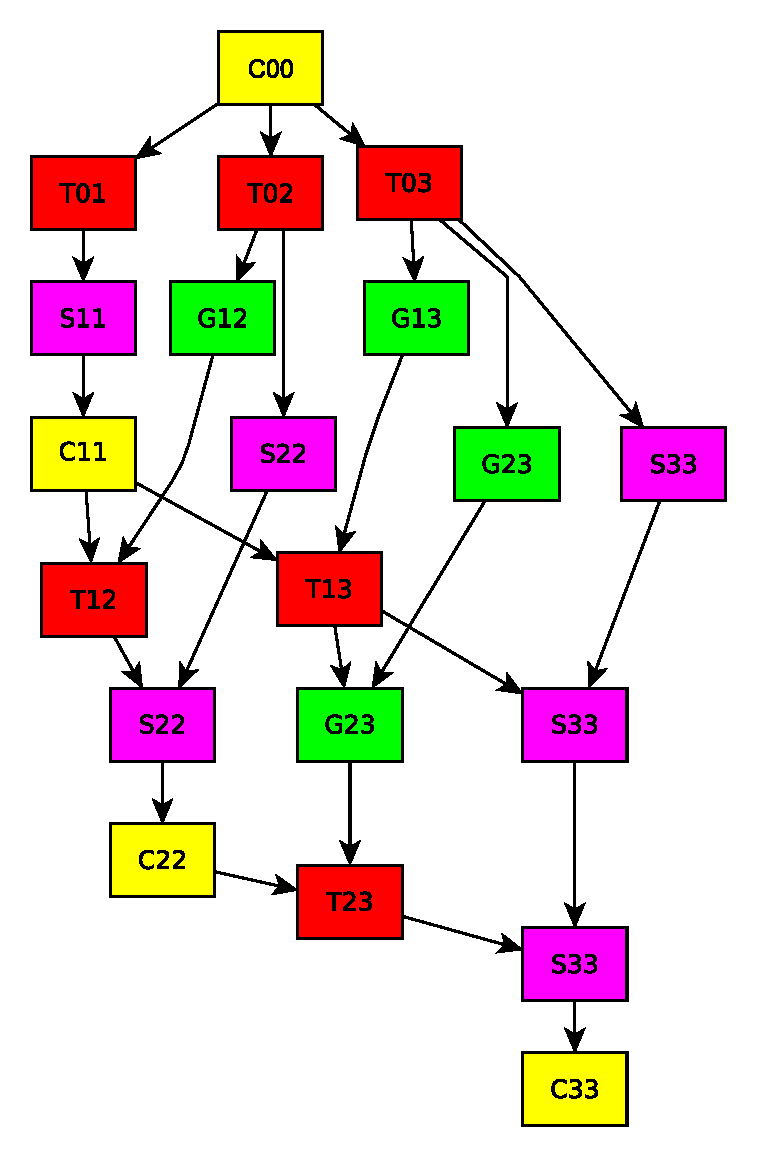
\includegraphics[scale=0.35]{Figures/4x4_TaskExample}
\end{center}
	\caption[DAG con las tareas y dependencias de datos resultantes de la aplicación del código en la Figura~\ref{lst:chol}
         sobre una matriz compuesta por $4 \times 4$ bloques ({\tt s}=4).]
	 {DAG con las tareas y dependencias de datos resultantes de la aplicación del código en la Figura~\ref{lst:chol}
         sobre una matriz compuesta por $4 \times 4$ bloques ({\tt s}=4). Las etiquetas especifican el tipo de kernel/tarea
         con la siguiente correspondencia: 
         ``{\sf C}'' para la Factorización de Cholesky,
         ``{\sf T}'' para la resolución de sistema triangular,
         ``{\sf G}'' para la multiplicación de matrices, y
         ``{\sf S}'' para la actualización simétrica de rango-{\tt b}. 
	 Los subíndices (comenzando en 0) especifican la submatriz que la tarea correspondiente actualiza.}
\label{fig:dag}
%\vspace{-0.5cm}
\end{figure}

El orden en el que dichos kernels son invocados durante la ejecución de la rutina, 
así como las submatrices o bloques que cada kernel lee o escribe, genera un grafo acíclico dirigido (DAG)
que refleja las dependiencias entre tareas (esto es, entre instancias de los kernels) y, por tanto,
el paralelismo de tareas potencial de la operación.
Por ejemplo, la Figura ~\ref{fig:dag} muestra el DAG con las tareas (nodos) y las dependencias de datos
(arcos) intrínsecas a la ejecución del código de la Figura~\ref{lst:chol}, cuando éste se ejecuta sobre
una matriz compuesta por $4 \times 4$ submatrices (esto es, cuando {\tt s}=4).  

El código de la Figura~\ref{lst:chol_tasks} muestra las anotaciones necesarias por parte del programador para explotar
el paralelismo a nivel de tareas inherente a la factorización de Cholesky usando OmpSs; cabe destacar las líneas etiquetadas
con  anotaciones (directivas) ``{\tt \#pragma omp task}''.
Las cláusulas {\tt in}, {\tt out} e {\tt inout} denotan la direccionalidad de los datos, y ayudan al planificador
de tareas a mantener coherentemente las dependencias entre tareas durante la ejecución. 
En esta implementación, los cuatro kernels anotados son implementados como invocaciones a 
kernels computacionales básicos de álgebra lineal proporcionados por LAPACK
({\tt dpotrf}) y BLAS ({\tt dtrsm}, {\tt dgemm} y {\tt dsyrk}).

\lstinputlisting[float=th!,frame=lines,caption=Tareas etiquetadas necesarias para la factorización de Cholesky por bloques.,label=lst:chol_tasks]{Codes/cholesky_tasks.c}

\subsection{Adaptación de OmpSs a arquitecturas asimétricas}
\label{s3:botlev}

En servidores equipados con uno o más aceleradores --por ejemplo,
procesadores gráficos--, versiones especializadas de los planificadores de
tareas que acompañan a OmpSs, StarPU, MAGMA, Kaapi y {\tt
  libflame}~\cite{libflameref} son capaces de planificar tareas a núcleos
de propósito general (CPUs en adelante) o a aceleradores (por ejemplo,
procesadores gráficos --GPUs-- o Intel Xeon Phi), asignando tareas a cada
tipo de recurso en función de sus propiedades, y aplicando técnicas como
caches gestionadas por software o mapeado de tareas explotando la localidad
de datos (véanse, entre
otros,~\cite{Quintana:2008:PMA,CPE:CPE1463,Augonnet:2011:SUP:1951453.1951454,5470941,Gautier:2013:XRS:2510661.2511383}). Este
tipo de adaptaciones, además, permiten la gestión transparente de
transferencias de datos entre distintos espacios de memoria, característica
principal en sistemas heterogéneos modernos.





%Recently OmpSs has been extended with a tailored scheduler for ARM big.LITTLE processors that 
%discriminates between the target being a fast (big) or a slow (LITTLE) core. This variant integrates uni- or bi-directional
%work stealing between the two types of cores, and specific criticality-aware mapping techniques~\cite{OmpSsbigLITTLE}. This runtime will be
%used as a base of our comparative experimental analysis in the experiments.

Con el reciente auge de las arquitecturas asimétricas en el mundo HPC, el
equipo de desarrollo de OmpSs ha introducido recientemente un nuevo
planificador denominado \emph{Bottom level-aware scheduler}
(Botlev)~\cite{botlev} específico para este nuevo tipo de
arquitecturas. Botlev recoge las ideas de los planificadores tradicionales
basados en arquitecturas heterogéneas, distinguiendo únicamente dos tipos
de nodos de cómputo (un nodo rápido formado por los cores de tipo big, y un
nodo de cómputo lento formado por los cores de tipo LITTLE) y eliminando el
cálculo de los costes asociados a
la transferencia de datos. \\

Una técnica utilizada para obtener un mejor rendimiento en programas
paralelos basados en tareas es intentar que las tareas críticas finalicen
su ejecución en el menor tiempo posible. Se denominan tareas críticas de un
DAG a aquellas tareas que en caso de retrasar su ejecución, producen un
retraso en la ejecución del problema. El planificador \botlev persigue este
objetivo intentando calcular de manera dinámica qué tareas pertenecen al
camino crítico del DAG asociado al problema, y ejecutar estas tareas sobre
cores rápidos con el objetivo de finalizar su ejecución cuanto
antes. Además, en caso de existir más tareas no críticas, las tareas
críticas tendrán preferencia frente a las tareas críticas. El objetivo de
garantizar que las tareas del camino crítico se ejecutan en los cores
rápidos cuanto antes es asegurarse que al ejecutar las tareas críticas,
estas liberarán dependencias con nuevas tareas que pasarán a estar listas
para ejecución, y así intentar conseguir que nunca haya \wts ociosos a
causa de que no existan tareas listas para ejecutar, lo cual disminuiría el
rendimiento global de la aplicación. La principal diferencia entre botlev y
los planificadores tradicionales para sistemas heterogéneos es que \botlev
toma las decisiones en tiempo dinámico sin necesidad de conocer de antemano
información sobre las tareas, o al forma del árbol de dependencias.

Para determinar si una tarea pertenece al camino crítico o no en tiempo de
ejecución, botlev asigna una prioridad a cada tarea en el momento de la
inserción en el grafo de dependencias, y la actualiza con la creación de
nuevas tareas. Una vez que la tarea está lista para ser ejecutada (es
decir, cuando todas las tareas que tenían relación con la tarea mediante el
grafo de dependencias han finalizado su ejecución), a partir de su
preferencia se realiza la decisión de si la tarea es considerada crítica o no.\\
La prioridad de una tarea viene dada por un número entero positivo, el cuál
representa la longitud del camino más largo desde la tarea actual hasta una
tarea hoja del grafo de dependencias. Cuando una tarea es introducida en el
DAG asociado al problema, se le asigna una prioridad 0 ya que la longitud
del camino más largo desde la tarea a un nodo hoja (ella misma) es
0. Además, cuando una nueva tarea es insertada en el árbol, se actualizan
todas las tareas predecesoras, ya que las prioridades de estas pueden haber
cambiado: por cada tarea predecesora, se intenta aumentar la prioridad en 1
unidad (el camino es un nodo más largo), siempre que no tuviera una
prioridad mayor antes (este es el caso de que la tarea pertenezca a un
camino más largo en el que la nueva tarea no esté involucrada). El proceso
de actualización finaliza cuando se actualiza la tarea raíz del árbol, o
cuando se alcanza una tarea que pertenece a otro camino más largo que el
actual. En la figura~\ref{s3:fig:botlev_tdg} se puede ver el camino crítico
detectado para una factorización de Cholesky sobre una matriz dividida en
$8\times8$ bloques. Hay que destacar que esta forma de calcular el camino
crítico detecta las tareas que pertenecen al camino más largo, pero eso no
implica que sean aquellas que más van a retrasar la ejecución en caso de
que no se ejecuten de manera prioritaria. Para calcular esto, sería
necesario conocer de antemano las necesidades de cada tarea, o ir
almacenando resultados parciales de ejecución de manera dinámica para tomar
decisiones en el futuro.

\begin{figure}
  \centering
  
  \begin{subfigure}{.45\textwidth}
    \centering
    \setlength{\fboxsep}{5pt}
    \fbox{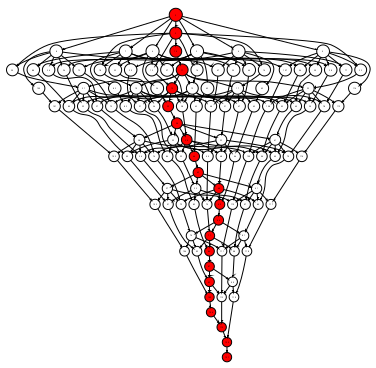
\includegraphics[width=.8\linewidth]{Figures/botlev-tdg.png}}
    \caption[Camino crítico en botlev para una factorización de Cholesky de
      $8\times8$ bloques]{Camino crítico en botlev para una factorización de Cholesky de
      $8\times8$ bloques. Fuente:~\cite{botlev}}
    \label{s3:fig:botlev_tdg}
  \end{subfigure}
  % Si se deja una línea en blanco, las coloca en vertical
  \begin{subfigure}{.47\textwidth}
    \centering
    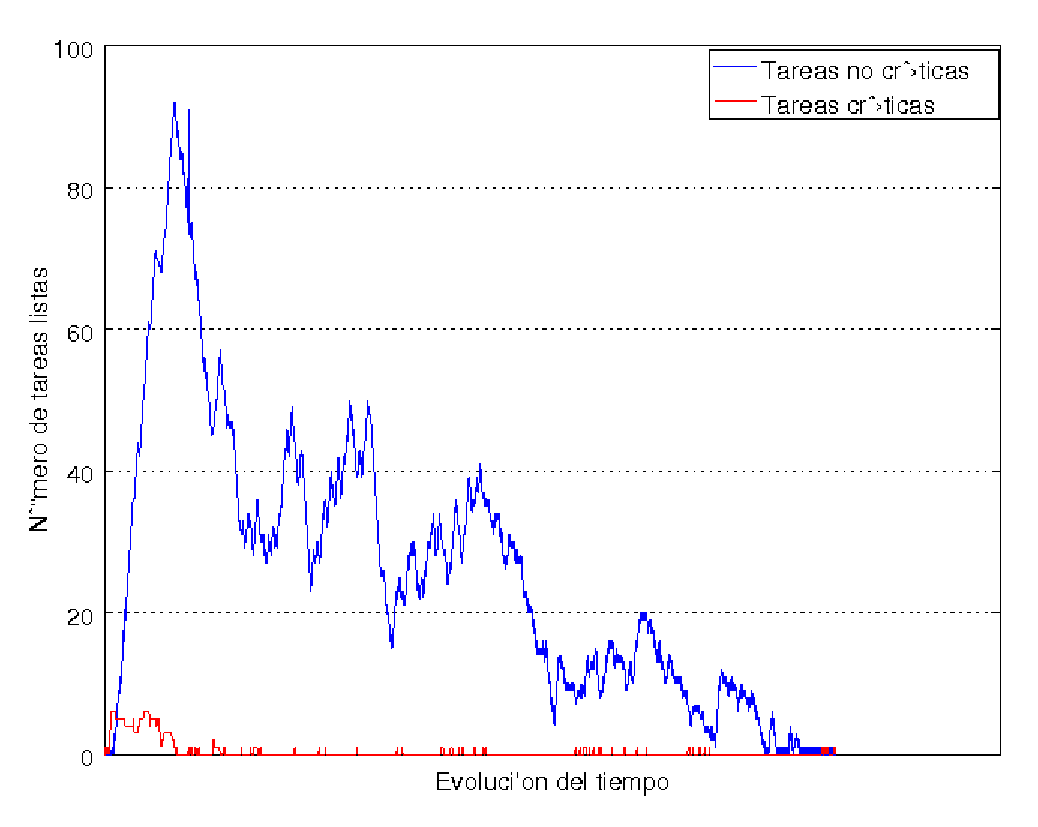
\includegraphics[width=1\linewidth]{Figures/botlev-colas.eps}
    \caption{Evolución del tamaño de las colas de tareas
      listas.}
    \label{s3:fig:botlev_colas}
  \end{subfigure}  
  
  \caption{Cálculo de tareas críticas en Botlev y asignación a cores.}
  \label{s3:fig:botlev}
\end{figure}

Una tarea puede ser ejecutada cuando todas sus tareas predecesoras han
finalizado la ejecución. Cuando esto ocurre, Botlev inserta la tarea en una
cola de tareas pendientes para ir ejecutándolas en función de la prioridad
asignada, o en orden de insercción en caso de empate. Estas tareas son
asignadas a los diferentes cores según vayan finalizando la ejecución de
las tareas previas. Según la prioridad de la tarea, Botlev distingue dos
tipos de colas en las que insertar una tarea: la cola con las tareas
pertenecientes al camino crítico, y la cola con el resto de tareas. Una
tarea se considera que pertenece al camino crítico si posee una prioridad
mayor a cualquiera de las prioridades de las tareas anteriores, o si es
hija directa de una tarea que se ha considerado crítica y tiene una
prioridad de una unidad menor (es decir, es el siguiente nodo del camino
crítico). En la figura~\ref{s3:fig:botlev_colas} se puede ver la evolución
del tamaño de las colas para una factorización de Cholesky sobre una matriz
de $8\times8$ bloques. La línea azul muestra el número de tareas no
críticas listas para ser ejecutadas en función del momento de la ejecución
del problema, mientras que la línea roja muestra el número de tareas
críticas. Como se puede apreciar, a mitad de ejecución el número de tareas
listas para ejecución disminuye considerablemente, y hasta que un conjunto
de tareas detectadas como críticas no son ejecutadas, el número de tareas
listas no vuelve a aumentar. Este es un ejemplo de cómo retrasar la
ejecución de una tarea crítica supone retrasar la creación de tareas, y por
tanto, tener un impacto negativo en el rendimiento.

Cuando un core big finaliza la ejecución de una tarea, este ejecutará la
siguiente tarea de la cola de tareas críticas, mientras que un core LITTLE
ejecutará la primera tarea de la cola de tareas no críticas. De esta forma
se consigue asignar las tareas críticas a cores big, mientras que las
tareas no críticas serán ejecutadas por cores lentos. Para grafos de
dependencias muy anchos, como puede ser el asociado a una factorización de
Cholesky, el número de tareas críticas es mucho menor que el número de
tareas no críticas, dando lugar a que los cores rápidos estén la mayor
parte de tiempo ociosos. Para evitar esta situación, si un core big no
dispone de tareas críticas que ejecutar, ejecutará la siguiente tarea de la
lista de tareas no críticas. El robo de tareas en sentido contrario (es
decir, que los cores LITTLE ejecuten tareas críticas) es una parámetro
adicional que se puede seleccionar en tiempo de ejecución, pero que se
encuentra desactivado por defecto.




%The designers/developers
%of the OmpSs programming model and the Nanos++ runtime task scheduler recently introduced a new version of their framework,
%hereafter referred to as Botlev-OmpSs,
%specifically tailored for AMPs~\cite{OmpSsbigLITTLE}. 
%This asymmetry-conscious runtime embeds a scheduling policy
%CATS (Criticality-Aware Task Scheduler) that relies on bottom-level longest-path priorities,
%keeps track of the criticality of the individual tasks, and leverages this information, at execution time, to 
%assign a ready task to either a critical or a non-critical queue. 
%In this solution, tasks enqueued in the critical queue can only be executed by the fast cores.
%In addition, the enhanced scheduler integrates uni- or bi-directional work stealing between fast and slow cores.
%According to the authors, this sophisticated {\em ad-hoc} scheduling strategy for heterogeneous/asymmetric processors attains remarkable performance
%improvements in a number of target applications; see~\cite{OmpSsbigLITTLE} for further details.
%
%When applied to a task-parallel DLA routine, the asymmetry-aware scheduler in Botlev-OmpSs
%maps each task to a single (big or LITTLE) core, and simply invokes a sequential DLA library to conduct the actual work.
%On the other hand, we note that this approach required an important redesign of the underlying scheduling policy (and thus, a considerable
%programming effort for the runtime developer), in order to exploit the heterogeneous architecture.
%In particular, detecting the criticality of a task at execution time is a nontrivial question.

%%{\bf Explain}



\section{Implementación paralela de bibliotecas matemáticas}
\label{sec:bibliotecas}

\subsection{BLIS: implementación multihebra del estándar BLAS}

A la hora de explotar el paralelismo potencial de una arquitectura, una segunda alternativa al efoque 
basado en planificación a nivel de tareas (es decir, explotando paralelismo
a nivel de tareas) consiste en el uso de kernels ya paralelizados, es decir, implementaciones
de rutinas que particionan estáticamente el trabajo entre los recursos computacionales existentes, o 
lo hacen aprovechando mecanismos sencillos de planificación como aquellos ofrecidos por OpenMP. Desde
este punto de vista, el paralelismo no se extrae ya a nivel de tarea, sino a nivel de datos, de forma
interna a cada tarea. Por ejemplo, en el ámbito del álgebra lineal, donde las dependencias de datos
internos a cada tarea es sencilla, o cuando el número de núcleos en el sistema es reducido, esta 
opción típicamente conlleva menos sobrecarga en tiempo de ejecución, y por tanto proporciona
una solución más eficiente desde el punto de vista del rendimiento. A día de hoy, esta es la
opción preferida y adoptada en bibliotecas comerciales y de software libre, como por ejemplo
AMD ACML~\cite{ACML}, IBM ESSL~\cite{ESSL}, Intel MKL~\cite{mkl}, GotoBLAS~\cite{Goto:2008:AHP}, OpenBLAS~\cite{OpenBLAS} o BLIS~\cite{BLIS1}. Todas estas bibliotecas son implementaciones
optimizadas de los estándares BLAS~\cite{blas1,blas2,blas3} y LAPACK~\cite{lapack}.

A modo de ejemplo, y dado que utilizaremos BLIS como biblioteca subyacente para la ejecución de tareas
individuales durante el resto del trabajo, se describe brevemente su funcionamiento, así como la posibilidad
de adaptar su paralelización a una arquitectura asimétrica.

BLIS implementa el enfoque algorítmico introducido por la biblioteca de álgebra lineal GotoBLAS, ampliamente
utilizada a día de hoy en multitud de arquitecturas. Este enfoque plantea la implementación de todas las rutinas
BLAS de nivel 3 (incluyendo el producto de matrices, \gemm) como tres bucles anidados sobre dos rutinas de 
empaquetado de datos, cuya finalidad es dirigir bloques de los operandos fuente a través de la jerarquía
de memoria, y un {\em macro-kernel} cuya función es la ejecución de las operaciones aritméticas asociadas
a cada operación. Internamente, BLIS implementa dicho macro-kernel como dos bucles adicionales sobre un 
{\em micro-kernel} que, a su vez, está formado por un bucle sobre una actualización de rango 1.

Para la siguiente descripción, únicamente consideraremos los tres bucles externos en la implementación de 
BLIS para \gemm, para el producto $C:=C+A\cdot B$, donde $A,B,C$ son matrices de dimensión $m \times k$, $k\times n$ 
y $m \times n$ respectivamente, almacenadas en los arrays {\tt A}, {\tt B} y {\tt C}; véase el código de la Figura~\ref{lst:gemm}.
En dicho código, {\tt mc}, {\tt nc}, {\tt kc} con parámetros de configuradción que necesitan ser sintonizados para cada
arquitectura teniendo en cuenta, entre otros, factores como la latencia de las unidades de punto flotante, número
de registros vectoriales y tamaño/grado de asociatividad de cada nivel de cache~\cite{BLIS4}.

\lstinputlisting[float=th!,frame=lines,caption=Implementación de altas prestaciones de \gemm en BLIS.,label=lst:gemm]{Codes/gemm.c}

\subsection{Implementación multihebra consciente de la asimetría}

La implementación de \gemm\ en BLIS obtiene un rendimiento cercano al rendimiento pico de la arquitectura,
tanto en sistemas multinúcleo como sistemas aceleradores~\cite{BLIS2,BLIS3}. 
Estos estudios han derivado en versiones de la implementación conscientes de la asimetría sobre arquitecturas ARM big.LITTLE
bajo el modelo de ejecución GTS. Concretamente, versión multihebra consciente de la asimetría descrita en~\cite{asymBLIS} 
integra las siguientes tres técnicas:
\begin{itemize}
\item Un particionado dinámico 1-D del espacio de iteraciones para distribuir la carga de los bucles~1 y~3 sobre los dos
	clusters (big y LITTLE).
\item Un particionado estático 1-D del espacio de iteraciones para distribuir la carga de uno de los  bucles internos entre los núcleos
	del mismo cluster.
\item Una modificación de los árboles de control que gobiernan la paralelización multihebra en BLIS para utilizar distintos {\em strides} en 
	los bucles, de modo que éstos se adapten a cada una de las arquitecturas subyacentes.
\end{itemize}

En general, esta estrategia puede ser aplicada a AMPs genéricos, consistentes en cualquier combinación de núcleos lentos y rápidos, y a cualquiera
de las rutinas BLAS implementadas en la biblioteca. Así, BLIS se convierte en una biblioteca que implementa rutinas básicas de álgebra lineal que,
internamente, explotan la asimetría de la arquitectura subyacente; esta característica será aprovechada en el resto del trabajo en combinación
con planificadores de tareas ``clásicos'' (no conscientes de la asimetría), como se describe en la siguiente sección.


\section{Paralelismo a nivel de tareas y a nivel de datos: ventajas e inconvenientes}
\label{sec:comparativa}

Existen pues dos alternativas principales a la hora de portar una determinada implementación (en nuestro caso, de una operación
de álgebra lineal) a una plataforma asimétrica:

\begin{enumerate}
 \item Utilizar un planificador de tareas consciente de la asimetría, en el que, por ejemplo, las tareas pertenecientes al camino crítico 
	 sean asignadas a núcleos de procesamiento rápidos. De este modo, la unidad básica de planificación de tareas es el núcleo individual,
		las tareas son invocaciones a versiones secuenciales de una determinada biblioteca, 
		y es el planificador de tareas el encargado de explotar en tiempo de ejecución, sin la intervención del programador, los
		núcleos asimétricos subyacentes.
		
	\item Utilizar una implementación de rutinas de biblioteca conscientes de la asimetría, sin extraer paralelismo a nivel de tareas. Una
		determinada invocación a una de estas rutinas se ejecutará eficientemente de forma paralela teniendo en cuenta las 
		características de la arquitectura asimétrica subyacente, repartiendo su espacio de iteraciones, por ejemplo, según las
		capacidades de cómputo de cada tipo de núcleo disponible.
\end{enumerate}

Las ventajas de la utilización de un planificador de tareas son obvias: menor intervención por parte del programador o usuario,
adaptación a pequeños cambios en el comportamiento dinámico de la arquitectura ante la ejecución de un código, o modificación
de las políticas de planificación dinámicamente, entre otras. Sin embargo, en muchas ocasiones, el sobrecoste de este tipo de
mecanismos no es desdeñable; además, su adaptación a arquitecturas heterogéneas o asimétricas, como es el caso, requiere
un desarrollo específico de nuevas políticas de planificación que exploten los recursos disponibles de manera eficiente.

Una biblioteca de funciones específicamente desarrollada para una arquitectura asimétrica (por ejemplo, BLIS en el ámbito del álgebra lineal) elimina gran parte
de este sobrecoste y suele conseguir mejores y más predecibles rendimientos, especialmente en arquitecturas no homogéneas. Sin
embargo, su desarrollo conlleva implementaciones específicas para cada tipo de arquitectura, lo que supone un esfuerzo no despreciable.

En el siguiente capítulo, se propone una solución que combina las ventajas de cada uno de los dos enfoque: combinando un planificador
no consciente de la asimetría (es decir, convencional) con una biblioteca para la ejecución de tareas optimizada para arquitecturas
asimétricas, se consigue aunar facilidad de programación y uso --derivado del uso de un planificador de tareas estándar-- con altas
prestaciones --derivadas de la utilización de una biblioteca desarrollada ad-hoc para este tipo de arquitecturas--.

%-- Configuraciones para emacs --
%%% Local Variables:
%%% mode: latex
%%% TeX-master: "./principal.tex"
%%% End:
